% Drawing 33/08-1 -- folder 33, batch 08, archive page 151 (PDF page 152).
% Transcription: au bas de la page, un réseau de lignes obliques entrecroisées (une rangée de losanges) sur lequel il a écrit en travers : « Dire », « $X$, $Y$ \uncertain{lisses} », « $F_\bullet$, $G_\bullet$ », « \uncertain{revient} \uncertain{à} \uncertain{dire} … \uncertain{d'habitude} », « $i_!(A_U)$, $j_!(A_V)$ », « $i : U\to X$, $j : V\to X$ », « $U$, $V$ », « \ill{} ». Le dessin et l'écriture paraissent superposés ; l'ordre de lecture n'est pas sûr.
% Kind: network of crossing oblique lines (row of lozenges) with words written across. Method 2 (schematic redraw from the facsimile). Status: partial.
% Notes: A row of lozenges made by rising and falling oblique lines, schematised as a regular lattice (eight apexes); the real lines are irregular and their number and spacing are approximate. The words written across are placed roughly where they are: "Dire", "X, Y", F, G, i_!(A_U), j_!(A_V), U, V, i : U -> X, j : V -> X; the uncertain phrase "revient a dire ... d'habitude" and the illegible word are left out.
% Coordinates: 1 unit = 1 mm = 1/100 of the crop width (bbox in page fractions: [0.08, 0.7, 0.94, 0.89]).
% Redrawn by Claude (claude-opus-5-5), issue #73, 2026-11-07; not checked by a human; not compiled (no TeX in the session).
% Rights: reproduces part of the work -- behind RENDER_TRANSCRIPTS, never published by itself.
\documentclass[tikz,border=3pt]{standalone}
\usepackage{amsmath,amssymb}
\usetikzlibrary{patterns,arrows.meta}
\tikzset{pencil/.style={black!45}, struck/.style={black!35}, mark/.style={circle,draw,inner sep=1.3pt}, pt/.style={circle,fill,inner sep=0.9pt}, opt/.style={circle,draw,fill=white,inner sep=1.1pt}}
\begin{document}
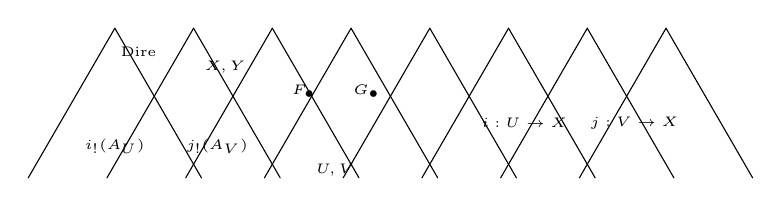
\begin{tikzpicture}[x=1mm,y=1mm,line cap=round,line join=round,font=\scriptsize]
\draw (7,-27) -- (18,-8);
\draw (17,-27) -- (28,-8);
\draw (27,-27) -- (38,-8);
\draw (37,-27) -- (48,-8);
\draw (47,-27) -- (58,-8);
\draw (57,-27) -- (68,-8);
\draw (67,-27) -- (78,-8);
\draw (77,-27) -- (88,-8);
\draw (18,-8) -- (29,-27);
\draw (28,-8) -- (39,-27);
\draw (38,-8) -- (49,-27);
\draw (48,-8) -- (59,-27);
\draw (58,-8) -- (69,-27);
\draw (68,-8) -- (79,-27);
\draw (78,-8) -- (89,-27);
\draw (88,-8) -- (99,-27);
\node[inner sep=1pt] at (21,-11) {\tiny Dire};
\node[inner sep=1pt] at (32,-13) {\tiny $X,Y$};
\node[inner sep=1pt] at (42,-16) {\tiny $F_\bullet$};
\node[inner sep=1pt] at (50,-16) {\tiny $G_\bullet$};
\node[inner sep=1pt] at (18,-23) {\tiny $i_!(A_U)$};
\node[inner sep=1pt] at (31,-23) {\tiny $j_!(A_V)$};
\node[inner sep=1pt] at (46,-26) {\tiny $U,V$};
\node[inner sep=1pt] at (70,-20) {\tiny $i:U\to X$};
\node[inner sep=1pt] at (84,-20) {\tiny $j:V\to X$};
\end{tikzpicture}
\end{document}
